\documentclass[12pt,aspectratio=169]{beamer}
\usepackage[utf8]{inputenc}
\usepackage[T1]{fontenc}
\usepackage[czech]{babel}
\usepackage{lmodern}
%\usetheme{Malmoe}
\usetheme{Fedora169}
\usepackage{graphicx}
\usepackage{newverbs}

\newverbcommand{\tc}{\color{blue}}{}

%\usebackgroundtemplate{\includegraphics[width=\paperwidth,height=\paperheight]{./images/background.jpg}}

\begin{document}
	\author{Lukáš Růžička (lruzicka@redhat.com)}
	\title{OpenQA testing platform}
	\subtitle{Train your own testing pet}
	\institute{Fedora QE}
	\date{April 2020}
	\setbeamertemplate{navigation symbols}{}

\begin{frame}[plain]
	\maketitle 
\end{frame}

\section{What is openQA}

\begin{frame}{What is openQA?}

\textbf{openQA} is an automated test tool, developed by SuSE, that allows to test various features of operating systems using the \textit{hands-on} approach:

\vspace{15pt}

\begin{itemize}
\item it runs the operating system
\item it provides an interface (console, GUI)
\item it takes input, passes it to the machine and triggers actions
\item it evaluates the reactions
\end{itemize}

\vspace{15pt}

It behaves similarly to a \textit{human} tester.
\end{frame}

\begin{frame}{Some technologies used}
	
	\begin{description}
		\item[qemu] runs the machines
		\item[VNC] provides the screens
		\item[perl scripts] define actions and evaluations
	\end{description}
\end{frame}

\begin{frame}{openQA architecture}
	\begin{description}
		\item[Controller]
			\begin{itemize}
				\item Web UI (control and visualization)
				\item job handling (scheduling, starting, stopping)
				\item live viewing and interaction (monitoring and development)
				\item results
				\item database (postgresql)
			\end{itemize}
		\item[Worker]
			\begin{itemize}
				\item assets (iso or qcow2)
				\item tests and needles 
				\item syncing and caching 
				\item video recording
			\end{itemize}
	\end{description}
\end{frame}

\begin{frame}{openQA architecture diagram}
	\begin{center}
		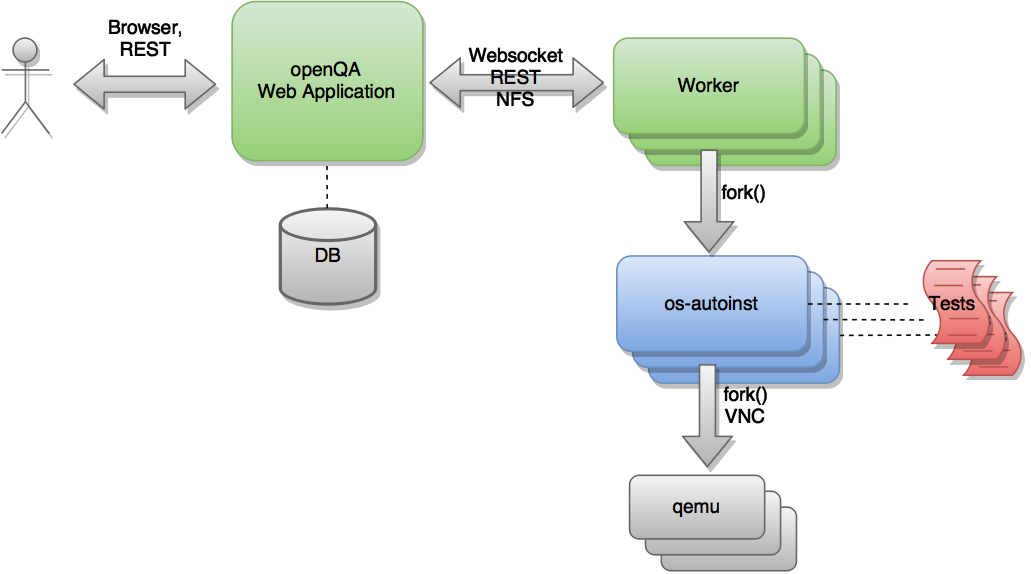
\includegraphics[width=12cm]{architecture}
	\end{center}
\end{frame}

\section{Concepts}

\begin{frame}{Basic concepts}
	\begin{itemize}
		\item machine
		\item tests grouping
		\item image
		\item job
		\item test suite
		\item test
		\item needle
	\end{itemize}
\end{frame}

\begin{frame}[fragile]{Machine}
	A \textbf{machine} is a qemu based virtual machine created with various settings. The following example shows the predefined \textbf{UEFI x86\_64} machine. 
	
	\vspace{5pt}
	
	\begin{verbatim}
	ARCH_BASE_MACHINE=64bit
	PART_TABLE_TYPE=gpt
	QEMUCPU=Nehalem
	QEMUCPUS=2
	QEMURAM=2048
	QEMUVGA=virtio
	QEMU_VIRTIO_RNG=1
	UEFI=1
	UEFI_PFLASH_CODE=/usr/share/edk2/ovmf/OVMF_CODE.fd
	UEFI_PFLASH_VARS=/usr/share/edk2/ovmf/OVMF_VARS.fd
	WORKER_CLASS=qemu_x86_64
	\end{verbatim}
	
\end{frame}

\begin{frame}[fragile]{Tests grouping}
	Single tests can be organized into groups according to several criteria and different test groups can be run for different images.
	\begin{description}
		\item[distri] a collection of definitions, perl functions, methods, tests, and needles, that covers the entire testing programme, such as \verb|os-autoinst-distri-fedora|
		\item[product] the main \textit{system under test} (SUT), such as \textbf{fedora} that is defined by a \textit{version}, \textit{flavor}, \textit{arch}, and has \textit{settings} assigned.
		\item[version] one version of a product, such as \textbf{Rawhide} or \textbf{32}.
		\item[flavor] a specific variant of a product to distinguish differing variants, e.g. \textbf{Workstation-live-iso}.
		\item[arch] an architecture variant of a product, e.g. \textbf{x86\_64}.
		\item[settings] variables to provide various settings, e.g. \verb|DESKTOP=gnome|.
	\end{description}
\end{frame}


\begin{frame}[fragile]{Image}
\textit{Images} are image files with the operating system to be tested. They are used to create and provide the virtual machines on which the actual tests are performed.

\vspace{5pt}

	\begin{itemize}
		\item iso $\longrightarrow$ qcow2
		\item qcow2
	\end{itemize}
\end{frame}

\begin{frame}[fragile]{Job}

is one \textit{physical} run of a \textit{test case} or a \textit{test suite}, defined as: \\
\textbf{{\tiny fedora-Rawhide-KDE-live-iso-x86\_64-BuildFedora-Rawhide-20200329.n.0-base\_service\_manipulation@64bit}}
 \vspace{5pt}
	
	\begin{itemize}
		\item product $\longrightarrow$ fedora
		\item version $\longrightarrow$ Rawhide
		\item flavor $\longrightarrow$ KDE-live-iso
		\item arch $\longrightarrow$ x86\_64
		\item build $\longrightarrow$ BuildFedora-Rawhide-20200329.n.0
		\item test suite $\longrightarrow$ base\_service\_manipulation
		\item machine $\longrightarrow$ 64bit
	\end{itemize}
\end{frame}

\begin{frame}[fragile]{Test Suite}

	a collection of several test cases that follow one another and together make sense, for example the \textbf{install\_default\_upload} test suite:	

	\vspace{5pt}
	
	\begin{enumerate}
		\item  \_boot\_to\_anaconda
		\item \_software\_selection
		\item disk\_guided\_empty
		\item \_do\_install\_and\_reboot
		\item \_graphical\_wait\_login
		\item \_collect\_data
		\item \_console\_shutdown
	\end{enumerate}
\end{frame}

\begin{frame}{A WebUI look on a test suite (job)}
	\begin{center}
		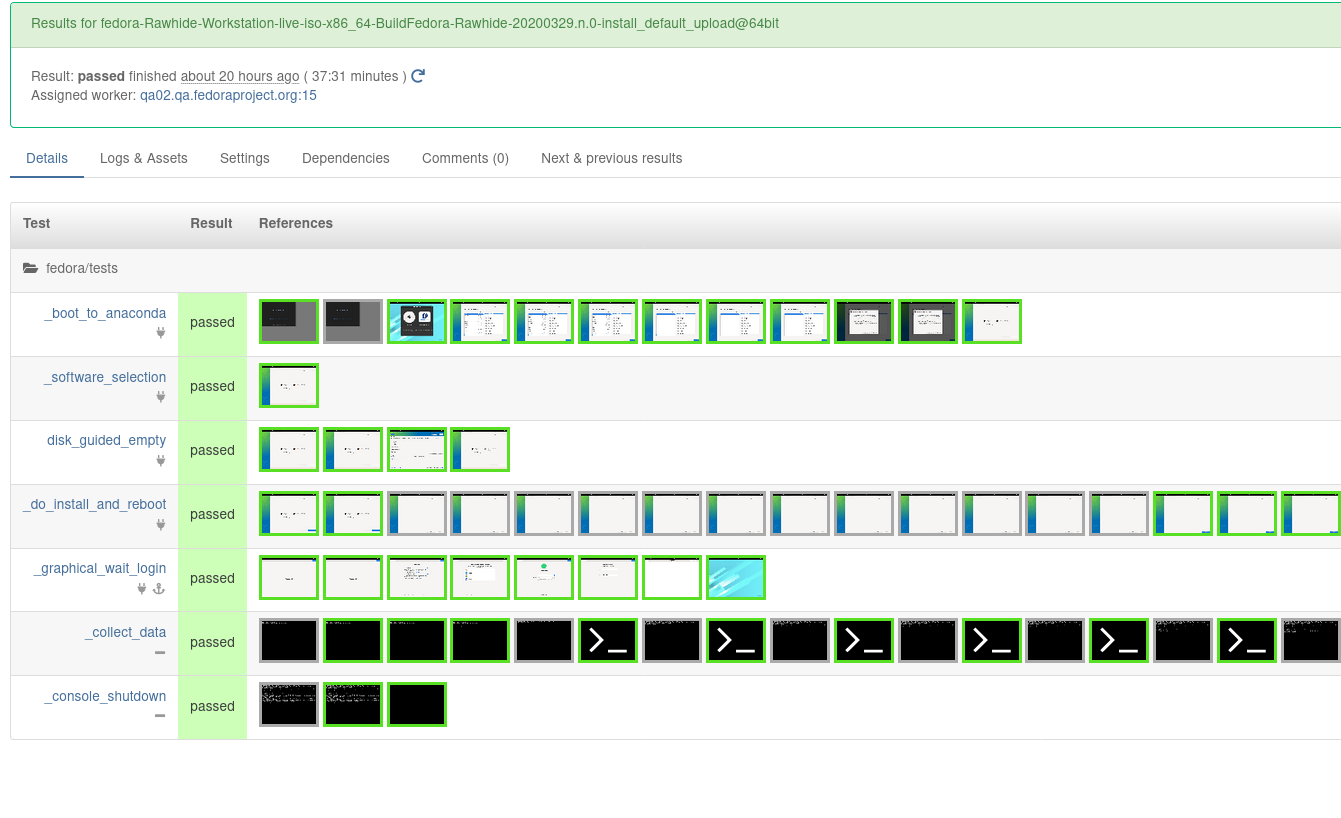
\includegraphics[width=12cm]{suite}
	\end{center}
\end{frame}

\begin{frame}{Test}
 	A \textbf{test} is a Perl script that defines what to do with the running virtual machine content and what to expect. 
 	
 	It mainly:
 	
 	\vspace{5pt}
		
	\begin{itemize}
		\item defines mouse actions
		\item defines keyboard actions
		\item checks and evaluates needles
		\item evaluates script outcomes
	\end{itemize}

	\vspace{5pt}
	
	The test (job) can have various \textit{statuses}, such as \textbf{passed}, \textbf{failed}, \textbf{softfailed}, \textbf{cancelled}, \textbf{running}, or \textbf{none}, etc.
\end{frame}

\begin{frame}[fragile]{Test example (Desktop Printing)}
	\begin{verbatim}
		# Open the text editor and print the file.
		wait_screen_change { send_key "alt-f2"; };
		wait_still_screen(stilltime=>5, similarity_level=>45);
		type_very_safely "$editor /home/test/testfile.txt\n";
		wait_still_screen(stilltime=>5, similarity_level=>44);
		
		# Print the file using the Cups-PDF printer
		send_key "ctrl-p";
		wait_still_screen(stilltime=>5, similarity_level=>45);
		if ($desktop eq 'gnome') {
		    assert_and_click "printing_select_pdfprinter";
		}
		else {
		    assert_screen "printing_pdfprinter_ready";
		}
	\end{verbatim}
\end{frame}

\begin{frame}{Needle}
	A \textbf{test} is a Perl script that defines what to do with the running virtual machine content and what to expect. 
	
	It mainly:
	
	\vspace{5pt}
	
	\begin{itemize}
		\item defines mouse actions
		\item defines keyboard actions
		\item checks and evaluates needles
		\item evaluates script outcomes
	\end{itemize}
	
	\vspace{5pt}
	
	The test (job) can have various \textit{statuses}, such as \textbf{passed}, \textbf{failed}, \textbf{softfailed}, \textbf{cancelled}, \textbf{running}, or \textbf{none}, etc.
\end{frame}

\end{document}